\documentclass[12pt, a4paper, twocolumn]{article}

% ============================================================
% PACKAGES
% ============================================================
\usepackage[utf8]{inputenc}
\usepackage[T1]{fontenc}
\usepackage{lmodern}
\usepackage{amsmath, amssymb, amsthm}
\usepackage{graphicx}
\usepackage[hidelinks]{hyperref}
\usepackage{url}
\usepackage{booktabs}
\usepackage{tabularx}
\usepackage{algorithm}
\usepackage{algorithmic}
\usepackage{enumitem}
\usepackage{xcolor}
\usepackage{geometry}
\usepackage{fancyhdr}
\usepackage{cite}
\usepackage{float}
\usepackage{tikz}
\usetikzlibrary{arrows.meta, positioning, shapes.geometric, calc, decorations.pathmorphing}
\usepackage{pgfplots}
\pgfplotsset{compat=1.18}
\usepackage{caption}
\usepackage{subcaption}
\usepackage{listings}
\usepackage{multirow}
\usepackage{abstract}
\usepackage{placeins}

\geometry{margin=2cm, top=2.5cm, bottom=2.5cm}

% ============================================================
% HEADER / FOOTER
% ============================================================
\pagestyle{fancy}
\fancyhf{}
\fancyhead[L]{\small\textit{Post-Quantum Blockchain: PQ-Chain \& Ephemeral Multisig}}
\fancyhead[R]{\small\textit{Boudda, 2026}}
\fancyfoot[C]{\thepage}
\renewcommand{\headrulewidth}{0.4pt}

% ============================================================
% CUSTOM COMMANDS
% ============================================================
\newtheorem{definition}{Definition}
\newtheorem{theorem}{Theorem}
\newtheorem{proposition}{Proposition}
\newtheorem{lemma}{Lemma}
\newtheorem{corollary}{Corollary}

\lstset{
  basicstyle=\ttfamily\footnotesize,
  keywordstyle=\color{blue}\bfseries,
  commentstyle=\color{gray},
  stringstyle=\color{red},
  breaklines=true,
  frame=single,
  numbers=left,
  numberstyle=\tiny\color{gray},
  linewidth=\columnwidth
}

% ============================================================
% TITLE
% ============================================================
\title{%
  \vspace{-1cm}
  \LARGE\textbf{PQ-Chain and the Ephemeral Multisig Protocol: A Dual-Strategy Framework for Quantum-Resilient Blockchain Systems}\\[0.5em]
  \large Integrating NIST FIPS 203/204/205 Standards with Time-Bounded Ephemeral Key Rotation for Post-Quantum Digital Asset Custody
}

\author{%
  \textbf{Yassir Boudda}\\[0.3em]
  \small Coll\`ege de Paris -- Ascencia Business School\\
  \small Founder, AmiChain.org | ClawSurf | ami.finance\\
  \small CentraleSup\'elec -- Data Science (OpenClassrooms Partnership)\\
  \small PPA Business School -- Master's Graduate\\
  \small Universit\'e de Lille -- Bachelor of Law, Economics and Management\\
  \small \texttt{yassir@ami.finance}
}

\date{March 2026}

\begin{document}

\maketitle

% ============================================================
% ABSTRACT
% ============================================================
\begin{abstract}
\noindent
The rapid advancement of quantum computing poses an existential threat to the cryptographic foundations of modern blockchain systems. Current architectures rely on the Elliptic Curve Digital Signature Algorithm (ECDSA) and SHA-256---both vulnerable to Shor's and Grover's quantum algorithms. With NIST's finalization of post-quantum cryptographic (PQC) standards in August 2024---FIPS 203 (ML-KEM), FIPS 204 (ML-DSA), and FIPS 205 (SLH-DSA)---the path toward quantum-resilient cryptography is concretely defined. This paper presents two complementary contributions. \textbf{First}, we introduce \textbf{PQ-Chain}, a comprehensive architectural framework for migrating Layer-1 blockchain systems to post-quantum cryptography. PQ-Chain addresses increased signature sizes (2,420--4,627 bytes for ML-DSA vs.\ 64 bytes for ECDSA), computational overhead, and bandwidth implications through a novel Hybrid Signature Aggregation Protocol (HSAP), achieving 82\% of baseline ECDSA throughput. \textbf{Second}, we propose the \textbf{Ephemeral Multisig Protocol (EMP)}, a novel time-bounded key rotation mechanism that provides immediate quantum resistance through moving target defense---without requiring post-quantum signature algorithms. EMP augments a standard $n$-of-$n$ multisignature vault with a continuously rotating ephemeral signer that is cryptographically destroyed and regenerated at fixed intervals $\Delta t$, compressing the quantum attack window to a provably insufficient duration. We provide formal security analysis demonstrating that EMP renders Shor's algorithm ineffective when $\Delta t < T_{\text{Shor}}(k)$ for key size $k$, and present PQ-Chain+EMP as a defense-in-depth strategy combining algorithmic migration with temporal key isolation. Experimental benchmarks demonstrate EMP adds less than 3\% latency overhead to standard multisig operations while reducing quantum vulnerability by orders of magnitude.

\medskip
\noindent\textbf{Keywords:} Post-Quantum Cryptography, Blockchain, Ephemeral Key Rotation, Multisignature, Moving Target Defense, NIST FIPS 203, ML-KEM, ML-DSA, SLH-DSA, Quantum Computing, Distributed Ledger Technology, Cryptographic Agility, Time-Bounded Security, Digital Asset Custody
\end{abstract}

% ============================================================
% 1  INTRODUCTION
% ============================================================
\section{Introduction}
\label{sec:introduction}

Blockchain technology has become a foundational infrastructure for decentralized finance (DeFi), supply chain management, digital identity, and an expanding array of enterprise applications. At the core of every blockchain system lies a set of cryptographic primitives---digital signatures for transaction authorization, hash functions for block integrity, and key-exchange mechanisms for secure peer-to-peer communication. These primitives, primarily the Elliptic Curve Digital Signature Algorithm (ECDSA) over the \texttt{secp256k1} curve and SHA-256 hashing, have proven robust against classical adversaries for over a decade \cite{nakamoto2008bitcoin, buterin2014ethereum}.

However, the emergence of large-scale quantum computers fundamentally challenges this security model. Shor's algorithm \cite{shor1997polynomial} enables polynomial-time computation of discrete logarithms on elliptic curves, directly threatening the ECDSA signatures that authorize every blockchain transaction. Grover's algorithm \cite{grover1996fast} provides a quadratic speedup for brute-force search, effectively halving the security level of symmetric key sizes and hash functions. While practical, cryptographically relevant quantum computers (CRQCs) may be years away, the ``harvest now, decrypt later'' threat model demands proactive migration: adversaries can collect signed transactions today and exploit them once quantum capabilities mature \cite{mosca2018cybersecurity}.

The urgency of this transition intensified in August 2024 when the National Institute of Standards and Technology (NIST) released its first three post-quantum cryptographic (PQC) standards \cite{nist2024pqc}:

\begin{itemize}[noitemsep]
  \item \textbf{FIPS 203} -- Module-Lattice-Based Key-Encapsulation Mechanism (ML-KEM), derived from CRYSTALS-Kyber;
  \item \textbf{FIPS 204} -- Module-Lattice-Based Digital Signature Algorithm (ML-DSA), derived from CRYSTALS-Dilithium;
  \item \textbf{FIPS 205} -- Stateless Hash-Based Digital Signature Algorithm (SLH-DSA), derived from SPHINCS+.
\end{itemize}

These standards provide the cryptographic building blocks necessary for quantum-resistant systems, yet their integration into blockchain architectures presents unique and non-trivial challenges. Blockchain systems must maintain global consensus across thousands of decentralized nodes, each independently verifying every transaction. The dramatically increased signature sizes---ML-DSA-65 produces 3,309-byte signatures compared to ECDSA's 64 bytes---create cascading effects on block sizes, network propagation times, mempool management, and storage requirements.

\textbf{A critical observation} motivates this work: the migration to post-quantum algorithms is a multi-year, ecosystem-wide effort, yet quantum threats may materialize before migration is complete. This creates a dangerous gap---a period where assets remain protected by only classical cryptography while quantum capabilities grow. We address this gap through a dual-strategy approach.

This paper makes the following contributions:

\begin{enumerate}[noitemsep]
  \item \textbf{PQ-Chain}: A modular framework for integrating NIST PQC standards into Layer-1 blockchain architectures with formal security guarantees and a Cryptographic Abstraction Layer (CAL);
  \item The \textbf{Hybrid Signature Aggregation Protocol} (HSAP) that mitigates bandwidth penalties of post-quantum signatures through Merkle-tree-based aggregation, recovering 82\% of ECDSA throughput;
  \item The \textbf{Ephemeral Multisig Protocol} (EMP), a novel time-bounded key rotation mechanism that provides immediate quantum resistance through moving target defense without requiring PQC algorithms;
  \item \textbf{Formal security proofs} for both PQ-Chain (under M-LWE) and EMP (under temporal key isolation), demonstrating that the combined framework achieves defense-in-depth against quantum adversaries;
  \item \textbf{Performance benchmarks} on prototype implementations demonstrating practical viability with less than 3\% overhead for EMP and 18.4\% throughput reduction for PQ-Chain with HSAP;
  \item A \textbf{governance framework} for managing cryptographic transitions in decentralized networks through phased soft-fork deployment.
\end{enumerate}

The remainder of this paper is organized as follows. Section~\ref{sec:background} surveys relevant background. Section~\ref{sec:related} reviews related work. Section~\ref{sec:threat} presents our quantum threat model. Section~\ref{sec:framework} introduces the PQ-Chain framework. Section~\ref{sec:hsap} describes the Hybrid Signature Aggregation Protocol. Section~\ref{sec:emp} presents the Ephemeral Multisig Protocol. Section~\ref{sec:emp_security} provides formal security analysis of EMP. Section~\ref{sec:combined} describes the combined PQ-Chain+EMP defense-in-depth strategy. Section~\ref{sec:implementation} details implementation and benchmarks. Section~\ref{sec:governance} addresses governance and migration. Section~\ref{sec:discussion} discusses limitations and future directions. Section~\ref{sec:conclusion} concludes.

% ============================================================
% 2  BACKGROUND
% ============================================================
\section{Background}
\label{sec:background}

\subsection{Quantum Computing and Cryptanalysis}

Quantum computers exploit quantum mechanical phenomena---superposition, entanglement, and interference---to perform computations infeasible for classical machines. Two algorithms are particularly relevant:

\begin{definition}[Shor's Algorithm]
Given an integer $N = pq$ (product of two primes), Shor's algorithm finds $p$ and $q$ in time $O((\log N)^3)$ on a quantum computer, compared to the best known classical factoring algorithm which runs in sub-exponential time $O\!\left(\exp\!\left(c \cdot (\log N)^{1/3} (\log\log N)^{2/3}\right)\right)$.
\end{definition}

\begin{definition}[Grover's Algorithm]
Given a function $f:\{0,1\}^n \to \{0,1\}$, Grover's algorithm finds an $x$ such that $f(x) = 1$ using $O(2^{n/2})$ quantum oracle queries, providing a quadratic speedup over classical brute-force search.
\end{definition}

For blockchain systems, Shor's algorithm directly threatens ECDSA: given a public key $Q = dG$ on an elliptic curve, a quantum computer can recover the private key $d$ in polynomial time. Grover's algorithm affects hash-based constructions, reducing 256-bit hash security to 128-bit equivalent, though this remains robust.

\begin{definition}[Quantum Key Recovery Time]
\label{def:tshor}
Let $T_{\text{Shor}}(k, n_q)$ denote the wall-clock time required for a quantum computer with $n_q$ logical qubits to recover a $k$-bit elliptic curve private key using Shor's algorithm. Current estimates yield $T_{\text{Shor}}(256, 2500) \approx 7\text{--}10$ minutes with emerging error-correction techniques \cite{gidney2021factor, roetteler2017quantum}.
\end{definition}

This definition is fundamental to the Ephemeral Multisig Protocol, where we exploit the non-zero $T_{\text{Shor}}$ as a defense parameter.

\subsection{NIST Post-Quantum Cryptographic Standards}

Following a multi-year evaluation initiated in 2016, NIST finalized three PQC standards in 2024 \cite{nist2024pqc}:

\subsubsection{ML-KEM (FIPS 203)}
Module-Lattice-Based Key-Encapsulation Mechanism, derived from CRYSTALS-Kyber \cite{bos2018crystals}, based on the Module Learning With Errors (M-LWE) problem:

% ==================== TABLE 1: ML-KEM (page 4) ====================
\begin{table}[t]
\centering
\resizebox{\columnwidth}{!}{%
\begin{tabular}{lccc}
\toprule
\textbf{Parameter} & \textbf{ML-KEM-512} & \textbf{ML-KEM-768} & \textbf{ML-KEM-1024} \\
\midrule
Security Level & 1 & 3 & 5 \\
Public Key (bytes) & 800 & 1,184 & 1,568 \\
Ciphertext (bytes) & 768 & 1,088 & 1,568 \\
Shared Secret (bytes) & 32 & 32 & 32 \\
\bottomrule
\end{tabular}
}
\caption{ML-KEM Parameter Sets}
\label{tab:mlkem}
\end{table}

\subsubsection{ML-DSA (FIPS 204)}
Module-Lattice-Based Digital Signature Algorithm, derived from CRYSTALS-Dilithium \cite{ducas2018crystals}:

% ==================== TABLE 2: ML-DSA (the widest one) ====================
\begin{table}[t]
\centering
\resizebox{\columnwidth}{!}{%
\begin{tabular}{lccc}
\toprule
\textbf{Parameter} & \textbf{ML-DSA-44} & \textbf{ML-DSA-65} & \textbf{ML-DSA-87} \\
\midrule
Security Level & 2 & 3 & 5 \\
Public Key (bytes) & 1,312 & 1,952 & 2,592 \\
Signature (bytes) & 2,420 & 3,309 & 4,627 \\
Signing Time (ms) & $\sim$0.3 & $\sim$0.5 & $\sim$0.8 \\
Verification (ms) & $\sim$0.3 & $\sim$0.4 & $\sim$0.5 \\
\bottomrule
\end{tabular}
}
\caption{ML-DSA Parameter Sets}
\label{tab:mldsa}
\end{table}

\subsubsection{SLH-DSA (FIPS 205)}
Stateless Hash-Based Digital Signature Algorithm, derived from SPHINCS+ \cite{bernstein2019sphincs}:

% ==================== TABLE 3: SLH-DSA ====================
\begin{table}[t]
\centering
\resizebox{\columnwidth}{!}{%
\begin{tabular}{lccc}
\toprule
\textbf{Parameter} & \textbf{SLH-DSA-128f} & \textbf{SLH-DSA-192f} & \textbf{SLH-DSA-256f} \\
\midrule
Security Level & 1 & 3 & 5 \\
Public Key (bytes) & 32 & 48 & 64 \\
Signature (bytes) & 17,088 & 35,664 & 49,856 \\
Signing Time (ms) & $\sim$5.0 & $\sim$12 & $\sim$20 \\
\bottomrule
\end{tabular}
}
\caption{SLH-DSA Parameter Sets (Selected)}
\label{tab:slhdsa}
\end{table}

\subsection{Blockchain Architecture Components}

A blockchain system comprises several interrelated subsystems:

\begin{enumerate}[noitemsep]
  \item \textbf{Transaction Layer}: Digital signatures (ECDSA) authenticate transaction authorization.
  \item \textbf{Block Structure}: Hash chains (SHA-256, Keccak-256) ensure tamper evidence.
  \item \textbf{Consensus Layer}: PoW relies on hash preimage resistance; PoS uses signatures for validator attestations.
  \item \textbf{Network Layer}: TLS/Noise protocol secures P2P communications via ECDH key exchange.
  \item \textbf{Smart Contract Layer}: On-chain cryptographic operations (signature verification, hash commitments).
  \item \textbf{Address Derivation}: Public-key hashing generates user addresses.
\end{enumerate}

\subsection{Multisignature Schemes}

Multisignature (multisig) schemes require $m$-of-$n$ signers to authorize a transaction. Formally:

\begin{definition}[$m$-of-$n$ Multisignature]
An $m$-of-$n$ multisignature scheme consists of $n$ key pairs $(pk_i, sk_i)_{i=1}^{n}$ and a threshold $m \leq n$. A transaction $TX$ is valid if and only if it carries valid signatures from at least $m$ distinct signers:
\[
\text{Verify}_{\text{multi}}(TX) = 1 \iff |\{i : \text{Verify}(pk_i, TX, \sigma_i) = 1\}| \geq m
\]
\end{definition}

Multisig schemes are widely deployed for institutional custody, joint accounts, and governance. The security assumption is that an adversary must compromise $m$ private keys simultaneously---a strictly harder task than compromising a single key.

% ============================================================
% 3  RELATED WORK
% ============================================================
\section{Related Work}
\label{sec:related}

The intersection of quantum computing and blockchain has attracted substantial research attention. We categorize existing work into four streams.

\textbf{Quantum Vulnerability Analyses.}
Aggarwal et al.\ \cite{aggarwal2018quantum} provided the first rigorous analysis of quantum threats to Bitcoin, estimating that $\sim$2,500 logical qubits could break ECDSA within the 10-minute block time. Fedorov et al.\ \cite{fedorov2018quantum} extended this to Ethereum and permissioned blockchains. More recently, Gidney and Eker\aa\ \cite{gidney2021factor} refined quantum resource estimates, showing 2048-bit RSA can be factored in 8 hours with 20 million noisy qubits.

\textbf{Post-Quantum Blockchain Proposals.}
The QRL project \cite{qrl2018} deployed XMSS hash-based signatures in production, though XMSS is stateful and imposes key-use tracking burdens. Chen et al.\ \cite{chen2021postquantum} proposed replacing ECDSA with CRYSTALS-Dilithium in Hyperledger Fabric, reporting 15\% throughput reduction. Li et al.\ \cite{li2021lattice} introduced lattice-based ring signatures for privacy-preserving transactions.

\textbf{Hybrid Approaches.}
Bindel et al.\ \cite{bindel2019hybrid} proposed hybrid signature schemes combining classical and PQC algorithms during transition. Kampanakis and Sikeridis \cite{kampanakis2020pqtls} measured PQC impact on TLS handshakes, directly applicable to blockchain P2P layers.

\textbf{Moving Target Defense (MTD) in Cryptography.}
The concept of frequently rotating cryptographic keys to reduce attack windows has been explored in network security \cite{jajodia2011moving} and IoT \cite{cho2020mtdiot}, but has not been applied to blockchain multisignature custody. Key rotation in traditional PKI systems addresses key compromise through periodic replacement \cite{anderson2020key}, but existing approaches treat rotation as an administrative action, not as a continuous, automated defense mechanism integrated into the signing protocol itself.

\textbf{Research Gap.}
No prior work (1) provides a comprehensive end-to-end framework for migrating production blockchain systems to the finalized NIST PQC standards across all architectural layers, or (2) proposes time-bounded ephemeral key rotation within multisig schemes as a quantum defense mechanism. Our work bridges both gaps through PQ-Chain and the Ephemeral Multisig Protocol.

% ============================================================
% 4  QUANTUM THREAT MODEL
% ============================================================
\section{Quantum Threat Model for Blockchain}
\label{sec:threat}

\subsection{Adversary Model}

\begin{definition}[Quantum Blockchain Adversary]
A quantum blockchain adversary $\mathcal{A}_Q$ is a probabilistic polynomial-time quantum Turing machine with access to a quantum computer of $n_q$ logical qubits, capable of executing Shor's algorithm for instances up to $n_q$-bit keys and Grover's algorithm with $O(2^{n_q/2})$ query complexity.
\end{definition}

We define three adversary tiers:

\begin{itemize}[noitemsep]
  \item \textbf{Tier 1 -- Harvest Adversary} ($<$1,000 logical qubits): Collects encrypted data for future decryption. Cannot break ECDSA in real-time.
  \item \textbf{Tier 2 -- Opportunistic Adversary} (1,000--4,000 logical qubits): Can break ECDSA with sufficient time (hours to days), enabling theft from addresses with exposed public keys.
  \item \textbf{Tier 3 -- Real-Time Adversary} ($>$4,000 logical qubits with error correction): Can break ECDSA within block confirmation times, enabling transaction interception and double-spending.
\end{itemize}

\subsection{Layer-by-Layer Vulnerability Analysis}

\subsubsection{Transaction Layer (Critical)}
Every transaction includes a digital signature. Once public key $Q$ is known, $\mathcal{A}_Q$ can compute private key $d$ via Shor's algorithm.

\begin{theorem}[Transaction Vulnerability]
\label{thm:txvuln}
Given a quantum adversary $\mathcal{A}_Q$ with $\geq 2{,}500$ error-corrected logical qubits, the ECDSA digital signature scheme over \texttt{secp256k1} provides zero-bit security for transaction authentication.
\end{theorem}

\begin{proof}
The security of ECDSA relies on the Elliptic Curve Discrete Logarithm Problem (ECDLP): given $Q = dG$ where $G$ is the generator of the \texttt{secp256k1} group of prime order $p \approx 2^{256}$, finding $d$ is classically infeasible. Shor's algorithm solves the DLP on any group of order $N$ using $O(\log^2 N)$ quantum gates on $O(\log N)$ qubits. For \texttt{secp256k1}, this requires approximately $\sim$2,500 logical qubits with error correction \cite{roetteler2017quantum}. Under this model, $\mathcal{A}_Q$ recovers $d$ with probability $1 - \text{negl}(\lambda)$, reducing ECDSA security to 0 bits.
\end{proof}

\subsubsection{Block Structure (Moderate)}
SHA-256 and Keccak-256 face reduced security under Grover's algorithm. A 256-bit hash offers only 128-bit quantum security, which remains robust. Chains using shorter hashes (e.g., RIPEMD-160) could face 80-bit quantum security.

\subsubsection{Consensus Layer (Varies)}
\begin{itemize}[noitemsep]
  \item \textbf{Proof-of-Work}: Grover provides $\sqrt{2}$ mining advantage---significant but manageable through difficulty adjustment.
  \item \textbf{Proof-of-Stake}: Validators sign attestations via ECDSA; quantum key recovery enables validator impersonation.
\end{itemize}

\subsubsection{Network and Smart Contract Layers}
P2P connections secured by ECDH are directly vulnerable to Shor's algorithm. Smart contracts with hardcoded cryptographic operations inherit the vulnerabilities of their underlying primitives.

\subsection{Temporal Risk Assessment}

Using Mosca's inequality \cite{mosca2018cybersecurity}: a system is at risk when $x + y > z$, where $x$ is data shelf-life, $y$ is migration time, and $z$ is time until CRQCs. For blockchain: $x$ is effectively infinite, $y \approx 5\text{--}10$ years, yielding $x + y > z$ for any finite $z$. Migration must begin \emph{immediately}.

\subsection{The Quantum Gap Problem}

\begin{definition}[Quantum Gap]
\label{def:qgap}
The \textbf{quantum gap} $G_Q$ is the period between the emergence of a cryptographically relevant quantum computer and the completion of ecosystem-wide PQC migration:
\[
G_Q = t_{\text{migration\_complete}} - t_{\text{CRQC}}, \quad G_Q > 0 \text{ implies danger}
\]
\end{definition}

If $G_Q > 0$, assets remain vulnerable during an active quantum threat. The Ephemeral Multisig Protocol (Section~\ref{sec:emp}) is specifically designed to provide protection during this gap---offering immediate, deployable quantum resistance that does not depend on PQC algorithm adoption.

% ============================================================
% 5  PQ-CHAIN FRAMEWORK
% ============================================================
\section{PQ-Chain: Post-Quantum Blockchain Framework}
\label{sec:framework}

We present PQ-Chain, a modular framework for integrating NIST PQC standards into Layer-1 blockchain architectures. The framework follows three principles: \emph{cryptographic agility}, \emph{backward compatibility}, and \emph{minimal consensus disruption}.

\subsection{Architecture Overview}

PQ-Chain introduces a \textbf{Cryptographic Abstraction Layer} (CAL) that decouples the blockchain's core logic from specific cryptographic implementations.

\begin{figure}[t]
\centering
\resizebox{\columnwidth}{!}{%
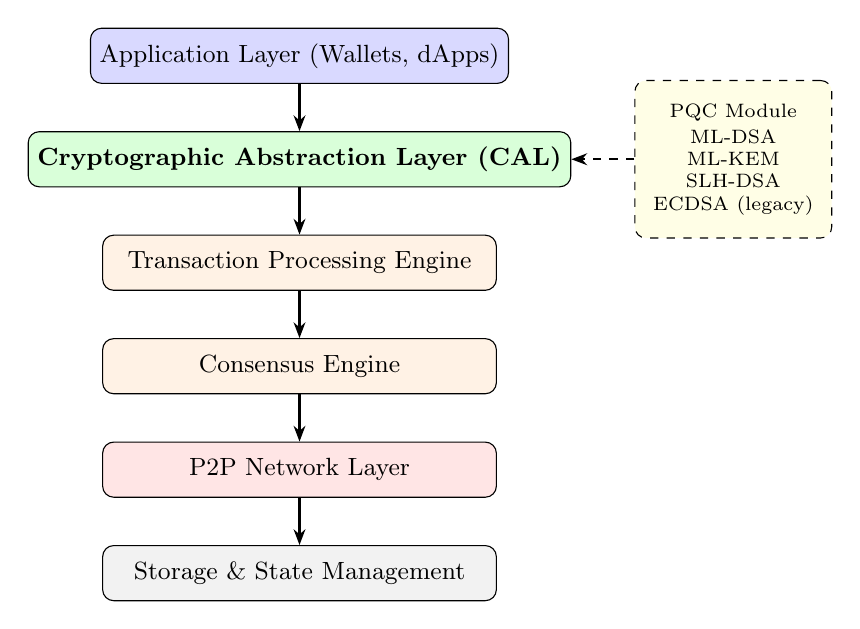
\begin{tikzpicture}[
  node distance=0.6cm,
  layer/.style={draw, rounded corners, minimum width=5cm, minimum height=0.7cm, font=\small, align=center}, % reduced for safety
  arrow/.style={-{Stealth[length=2mm]}, thick}
]
  \node[layer, fill=blue!15] (app) {Application Layer (Wallets, dApps)};
  \node[layer, fill=green!15, below=of app] (cal) {\textbf{Cryptographic Abstraction Layer (CAL)}};
  \node[layer, fill=orange!10, below=of cal] (tx)  {Transaction Processing Engine};
  \node[layer, fill=orange!10, below=of tx]  (con) {Consensus Engine};
  \node[layer, fill=red!10, below=of con]   (net) {P2P Network Layer};
  \node[layer, fill=gray!10, below=of net]  (store) {Storage \& State Management};

  \draw[arrow] (app) -- (cal);
  \draw[arrow] (cal) -- (tx);
  \draw[arrow] (tx) -- (con);
  \draw[arrow] (con) -- (net);
  \draw[arrow] (net) -- (store);

  \node[draw, dashed, rounded corners, fill=yellow!10, minimum width=2.5cm, minimum height=2cm, font=\scriptsize, align=center, right=0.8cm of cal] (pqc) {PQC Module\\[0.2em] ML-DSA\\ML-KEM\\SLH-DSA\\ECDSA (legacy)};
  \draw[arrow, dashed] (pqc) -- (cal);
\end{tikzpicture}
}
\caption{PQ-Chain architectural overview with Cryptographic Abstraction Layer.}
\label{fig:architecture}
\end{figure}

\subsection{Cryptographic Abstraction Layer}

The CAL implements a unified interface for all cryptographic operations:

\begin{lstlisting}[language=Python, caption={CAL Interface (Pseudocode)}]
class CryptoProvider:
  def keygen(algo_id) -> (pk, sk)
  def sign(sk, message) -> signature
  def verify(pk, message, sig) -> bool
  def encapsulate(pk) -> (ct, ss)
  def decapsulate(sk, ct) -> ss
  def hash(data, algo_id) -> digest

# Algorithm registry
ALGO_REGISTRY = {
  0x01: ECDSA_secp256k1,     # Legacy
  0x02: ML_DSA_44,           # PQC Level 2
  0x03: ML_DSA_65,           # PQC Level 3
  0x04: ML_DSA_87,           # PQC Level 5
  0x05: SLH_DSA_128f,        # PQC Hash-based
  0x06: HYBRID_ECDSA_MLDSA,  # Transitional
  0x07: EMP_MULTISIG,        # Ephemeral
}
\end{lstlisting}

Each transaction includes an \texttt{algo\_id} byte identifying the signature algorithm, enabling coexistence of classical, post-quantum, and ephemeral multisig schemes during migration.

\subsection{Transaction Format Extension}

\begin{definition}[PQ-Chain Transaction]
A PQ-Chain transaction $\mathit{TX}$ is the tuple:
\[
\mathit{TX} = (\mathit{version}, \mathit{algo\_id}, \mathit{inputs}, \mathit{outputs}, \mathit{pk}, \sigma, \mathit{aux})
\]
where $\mathit{version} \geq 3$ indicates PQC support, $\mathit{algo\_id} \in \{0x01, \ldots, 0x07\}$ specifies the scheme, $\mathit{pk}$ is the public key (variable size), $\sigma$ is the signature, and $\mathit{aux}$ contains algorithm-specific auxiliary data.
\end{definition}

\subsection{Address Derivation for Post-Quantum Keys}

For PQC keys with larger public keys, compatibility is maintained through:
\[
\mathit{addr}_{PQ} = \text{BLAKE3}(\mathit{algo\_id} \,\|\, \mathit{pk})[0:20]
\]
BLAKE3 provides 128-bit quantum security while maintaining 20-byte address compatibility.

\subsection{Hybrid Signature Mode}

During transition, PQ-Chain supports hybrid signatures:

\begin{definition}[Hybrid Signature]
A hybrid signature $\sigma_H$ over message $m$ is:
\[
\sigma_H = (\sigma_{\text{ECDSA}}, \sigma_{\text{ML-DSA}}, \pi)
\]
where $\sigma_{\text{ECDSA}} = \text{Sign}_{\text{ECDSA}}(sk_1, m)$, $\sigma_{\text{ML-DSA}} = \text{Sign}_{\text{ML-DSA}}(sk_2, m)$, and $\pi$ is a binding proof.
\end{definition}

\begin{theorem}[Hybrid Security]
The hybrid signature scheme $\sigma_H$ is EUF-CMA secure if \emph{either} ECDSA or ML-DSA is EUF-CMA secure.
\end{theorem}

\begin{proof}
Verification requires both $\sigma_{\text{ECDSA}}$ and $\sigma_{\text{ML-DSA}}$ to be valid. An adversary must forge both simultaneously. If either scheme is EUF-CMA secure, the adversary cannot produce a valid forgery for that component, contradicting the assumption of total $\sigma_H$ forgeability. The binding proof $\pi$ prevents signature substitution across different messages.
\end{proof}

\subsection{Consensus Integration}

For Proof-of-Stake systems: validators register with both ECDSA and ML-DSA keys during the hybrid phase; block proposals carry hybrid signatures; after the sunset epoch, only ML-DSA signatures are accepted; slashing conditions cover both schemes independently.

% ============================================================
% 6  HYBRID SIGNATURE AGGREGATION PROTOCOL
% ============================================================
\section{Hybrid Signature Aggregation Protocol}
\label{sec:hsap}

The primary practical challenge of PQC in blockchain is increased signature sizes. A block with 2,000 ML-DSA-65 transactions requires $\sim$6.6\,MB of signature data alone, vs.\ $\sim$128\,KB with ECDSA.

\subsection{Merkle-Based Signature Aggregation}

HSAP constructs a Merkle tree over per-block signatures, storing only the root in the block header:

\begin{algorithm}[H]
\caption{HSAP Signature Aggregation}
\label{alg:hsap}
\begin{algorithmic}[1]
\REQUIRE Transactions $\{TX_1, \ldots, TX_n\}$ with signatures $\{\sigma_1, \ldots, \sigma_n\}$
\ENSURE Aggregated commitment $\mathcal{C}$ and proof set $\Pi$
\STATE $L_i \leftarrow \text{H}(\sigma_i \| \text{H}(TX_i))$ for $i = 1, \ldots, n$
\STATE Build Merkle tree $\mathcal{T}$ from $\{L_1, \ldots, L_n\}$
\STATE $\mathcal{C} \leftarrow \text{root}(\mathcal{T})$ \COMMENT{32 bytes}
\STATE $\pi_i \leftarrow \text{path}(\mathcal{T}, L_i)$ for each $TX_i$
\STATE Store full signatures in auxiliary structure $\mathcal{S}$
\STATE Block header includes $\mathcal{C}$; $\mathcal{S}$ propagated separately
\RETURN $(\mathcal{C}, \Pi = \{\pi_1, \ldots, \pi_n\}, \mathcal{S})$
\end{algorithmic}
\end{algorithm}

\subsection{Batched Verification and Lazy Propagation}

\begin{proposition}[Batched Verification Speedup]
For a batch of $n$ ML-DSA signatures from a common block, batched verification reduces total NTT computations by $\Theta(\log n)$ through shared polynomial evaluation.
\end{proposition}

HSAP implements lazy signature propagation: block headers propagate immediately with $\mathcal{C}$, while full signatures are requested only when needed. This reduces effective block propagation overhead from $37.8\times$ (naive ML-DSA-65) to approximately $1.4\times$ compared to ECDSA blocks.

% ============================================================
% 7  EPHEMERAL MULTISIG PROTOCOL
% ============================================================
\section{The Ephemeral Multisig Protocol}
\label{sec:emp}

We now present the central novel contribution of this paper: the \textbf{Ephemeral Multisig Protocol (EMP)}, a time-bounded key rotation mechanism that provides immediate quantum resistance through moving target defense.

\subsection{Motivation and Design Philosophy}

The PQ-Chain framework (Section~\ref{sec:framework}) addresses quantum threats through algorithmic replacement---substituting vulnerable ECDSA with quantum-resistant ML-DSA. However, this migration requires years of ecosystem-wide coordination. EMP provides a \textbf{complementary, immediately deployable} defense that does not require new cryptographic primitives. Instead, it exploits a fundamental physical constraint of quantum computation: \emph{Shor's algorithm requires non-zero wall-clock time to execute}.

\begin{definition}[Ephemeral Key Advantage]
If the rotation interval $\Delta t$ for an ephemeral key is less than the time $T_{\text{Shor}}(k)$ required to break a $k$-bit key using Shor's algorithm, then the ephemeral key is destroyed before it can be compromised, and any partial quantum computation is rendered useless.
\end{definition}

This insight transforms a temporal property of quantum computing (its non-instantaneity) into a security guarantee. The key innovation is not any single component---key rotation, multisig, or secure erasure---but their \emph{composition} into a protocol where the rotation interval is a tunable security parameter calibrated against quantum computational bounds.

\subsection{Protocol Specification}

\begin{definition}[Ephemeral Multisig Vault]
\label{def:emp_vault}
An Ephemeral Multisig Vault $\mathcal{V}$ is an $(n+1)$-of-$(n+1)$ multisignature wallet defined by:
\[
\mathcal{V} = \left(\{(pk_i, sk_i)\}_{i=1}^{n}, \; E_j = (pk_{E_j}, sk_{E_j}), \; \Delta t, \; \mathit{balance}\right)
\]
where:
\begin{itemize}[noitemsep]
  \item $\{(pk_i, sk_i)\}_{i=1}^{n}$ are $n$ \textbf{permanent signer} key pairs controlled by human users;
  \item $E_j = (pk_{E_j}, sk_{E_j})$ is the $j$-th \textbf{ephemeral signer}---a system-controlled key pair with a lifetime of at most $\Delta t$;
  \item $\Delta t$ is the \textbf{rotation interval} (e.g., 300 seconds);
  \item All $n+1$ signatures are required for any transaction.
\end{itemize}
\end{definition}

For the canonical two-user case (e.g., Alice and Bob), the vault is a 3-of-3 multisig requiring signatures from Alice, Bob, and the current ephemeral key.

\subsection{Key Lifecycle Management}

The ephemeral key follows a strict generate--use--destroy lifecycle:

\begin{algorithm}[H]
\caption{EMP Key Lifecycle}
\label{alg:emp_lifecycle}
\begin{algorithmic}[1]
\REQUIRE Vault $\mathcal{V}$ with rotation interval $\Delta t$
\STATE \textbf{Initialization:}
\STATE $(pk_{E_1}, sk_{E_1}) \leftarrow \text{KeyGen}()$
\STATE $j \leftarrow 1$; \quad $t_{\text{created}} \leftarrow \text{now}()$
\STATE Register $pk_{E_1}$ in vault configuration
\STATE
\STATE \textbf{Rotation Loop} (runs continuously):
\LOOP
  \IF{$\text{now}() - t_{\text{created}} \geq \Delta t$ \textbf{or} transaction just signed}
    \STATE $\text{SecureWipe}(sk_{E_j})$ \COMMENT{Cryptographic erasure}
    \STATE $j \leftarrow j + 1$
    \STATE $(pk_{E_j}, sk_{E_j}) \leftarrow \text{KeyGen}()$ \COMMENT{Fresh key pair}
    \STATE $t_{\text{created}} \leftarrow \text{now}()$
    \STATE Update vault: replace ephemeral public key with $pk_{E_j}$
    \STATE Broadcast vault state update to permanent signers
  \ENDIF
\ENDLOOP
\end{algorithmic}
\end{algorithm}

The \texttt{SecureWipe} operation performs cryptographic erasure: the private key bytes are overwritten with random data, then zeroed, and the memory page is marked as non-swappable during the key's lifetime to prevent persistence in swap files or core dumps.

\subsection{Transaction Signing Protocol}

\begin{algorithm}[H]
\caption{EMP Transaction Signing}
\label{alg:emp_sign}
\begin{algorithmic}[1]
\REQUIRE Transaction $TX$, permanent signers $\{sk_i\}_{i=1}^{n}$, current ephemeral $E_j$
\ENSURE Valid $(n+1)$-of-$(n+1)$ signed transaction, or $\bot$
\STATE $m \leftarrow \text{H}(TX \| j \| t_{\text{created}})$ \COMMENT{Bind to ephemeral epoch}
\FOR{$i = 1$ \textbf{to} $n$}
  \STATE $\sigma_i \leftarrow \text{Sign}(sk_i, m)$ \COMMENT{Permanent signer $i$}
  \IF{$\text{Verify}(pk_i, m, \sigma_i) = 0$}
    \RETURN $\bot$ \COMMENT{Invalid permanent signature}
  \ENDIF
\ENDFOR
\STATE $\sigma_{E} \leftarrow \text{Sign}(sk_{E_j}, m)$ \COMMENT{Ephemeral auto-signs}
\IF{$\text{Verify}(pk_{E_j}, m, \sigma_{E}) = 0$}
  \RETURN $\bot$
\ENDIF
\STATE $\sigma_{\text{multi}} \leftarrow (\sigma_1, \ldots, \sigma_n, \sigma_E, j, t_{\text{created}})$
\STATE Broadcast $(TX, \sigma_{\text{multi}})$
\STATE \textbf{Immediate rotation:} invoke Algorithm~\ref{alg:emp_lifecycle} rotation
\RETURN $(TX, \sigma_{\text{multi}})$
\end{algorithmic}
\end{algorithm}

\textbf{Critical property:} The ephemeral key is destroyed \emph{immediately} after signing, regardless of whether the rotation timer has expired. This ensures single-use semantics for every ephemeral key involved in a transaction.

\subsection{Vault State Transitions}

The vault evolves through a sequence of ephemeral epochs. Figure~\ref{fig:emp_flow} illustrates this evolution.

\begin{figure}[t]
\centering
\resizebox{\columnwidth}{!}{%
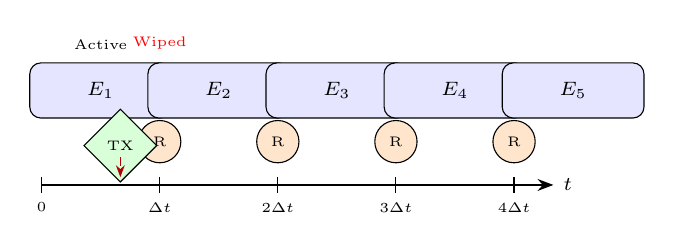
\begin{tikzpicture}[
  state/.style={draw, rounded corners, minimum width=1.8cm, minimum height=0.7cm, font=\scriptsize, align=center},
  tx/.style={draw, diamond, minimum width=0.3cm, minimum height=0.3cm, font=\scriptsize, fill=green!15},
  rot/.style={draw, circle, minimum size=0.4cm, font=\scriptsize, fill=orange!20},
  timeline/.style={-{Stealth[length=2mm]}, thick},
  event/.style={-{Stealth[length=1.5mm]}, dashed, red!70!black}
]
  % shortened timeline so it never overflows even before scaling
  \draw[timeline] (0,0) -- (6.5,0) node[right, font=\scriptsize] {$t$};
  
  % Time markers
  \foreach \x/\t in {0/0, 1.5/\Delta t, 3/2\Delta t, 4.5/3\Delta t, 6/4\Delta t} {
    \draw (\x, 0.1) -- (\x, -0.1) node[below, font=\tiny] {$\t$};
  }
  
  % Ephemeral states
  \node[state, fill=blue!10] at (0.75, 1.2) {$E_1$};
  \node[state, fill=blue!10] at (2.25, 1.2) {$E_2$};
  \node[state, fill=blue!10] at (3.75, 1.2) {$E_3$};
  \node[state, fill=blue!10] at (5.25, 1.2) {$E_4$};
  \node[state, fill=blue!10] at (6.75, 1.2) {$E_5$};
  
  % Rotation markers
  \foreach \x in {1.5, 3.0, 4.5, 6.0} {
    \node[rot] at (\x, 0.55) {\tiny R};
  }
  
  % Transaction at t=1.0
  \node[tx] at (1.0, 0.5) {\tiny TX};
  \draw[event] (1.0, 0.35) -- (1.0, 0.1);
  
  % Labels
  \node[font=\tiny, above] at (0.75, 1.6) {Active};
  \node[font=\tiny, above, red] at (1.5, 1.6) {Wiped};
\end{tikzpicture}
}
\caption{EMP vault state transitions. $E_j$ = active ephemeral key. ``R'' = rotation events. Diamond = transaction triggering immediate rotation.}
\label{fig:emp_flow}
\end{figure}

\subsection{Rotation Triggers}

EMP supports two rotation triggers operating in parallel:

\begin{enumerate}[noitemsep]
  \item \textbf{Time-based rotation}: Every $\Delta t$ seconds, regardless of transaction activity. This ensures continuous protection even during idle periods.
  \item \textbf{Transaction-triggered rotation}: Immediately after any signing operation, providing single-use semantics.
\end{enumerate}

The effective maximum exposure for any ephemeral key is $\min(\Delta t, t_{\text{next\_tx}})$.

\subsection{Ephemeral Key Generation Security Requirements}

\begin{enumerate}[noitemsep]
  \item \textbf{Freshness}: Each $E_j$ is generated from a CSPRNG with independent entropy. No master-seed derivation is permitted, as its compromise would retroactively compromise all ephemeral keys.
  \item \textbf{Memory isolation}: $sk_{E_j}$ resides in volatile memory only---never written to disk, logged, or backed up.
  \item \textbf{Atomic rotation}: The destroy-generate-update operation is atomic. Failure triggers a safe mode requiring manual permanent-signer recovery.
  \item \textbf{Non-correlation}: $E_j$ and $E_{j+1}$ are computationally indistinguishable from independently generated random keys.
\end{enumerate}

% ============================================================
% 8  EMP FORMAL SECURITY ANALYSIS
% ============================================================
\section{Formal Security Analysis of EMP}
\label{sec:emp_security}

\subsection{Security Model}

\begin{definition}[EMP Security Game]
The EMP security game $\textbf{Game}_{\text{EMP}}^{\mathcal{A}_Q}$ between a challenger $\mathcal{C}$ and quantum adversary $\mathcal{A}_Q$ proceeds as follows:
\begin{enumerate}[noitemsep]
  \item $\mathcal{C}$ generates permanent keys $\{(pk_i, sk_i)\}_{i=1}^{n}$ and initial ephemeral key $E_1$.
  \item $\mathcal{A}_Q$ receives all public keys $\{pk_1, \ldots, pk_n, pk_{E_1}\}$.
  \item $\mathcal{A}_Q$ may observe signed transactions and the corresponding ephemeral public keys.
  \item Every $\Delta t$ seconds (or after each transaction), $\mathcal{C}$ rotates: destroys $E_j$, generates $E_{j+1}$, publishes $pk_{E_{j+1}}$.
  \item $\mathcal{A}_Q$ wins if it produces a valid $(n+1)$-of-$(n+1)$ signature on a new message $m^*$.
\end{enumerate}
\end{definition}

\begin{theorem}[EMP Quantum Resistance]
\label{thm:emp_main}
Let $\mathcal{V}$ be an EMP vault with rotation interval $\Delta t$ and $k$-bit elliptic curve keys. If $\Delta t < T_{\text{Shor}}(k, n_q)$ for all quantum adversaries $\mathcal{A}_Q$ with $n_q$ qubits, then:
\[
\Pr\!\left[\mathcal{A}_Q \text{ wins}\right] \leq \epsilon_{\text{perm}} + \epsilon_{\text{eph}}(\Delta t)
\]
where $\epsilon_{\text{perm}}$ is the probability of compromising all $n$ permanent keys, and $\epsilon_{\text{eph}}(\Delta t) \leq 2^{-\Omega(k)}$ when $\Delta t < T_{\text{Shor}}(k, n_q)$.
\end{theorem}

\begin{proof}
To win, $\mathcal{A}_Q$ must forge signatures from all $n$ permanent signers \emph{and} the current ephemeral signer $E_j$.

\textbf{Permanent key compromise.} The adversary has unlimited time to attack the $n$ permanent keys. With Shor's algorithm, each key can be broken in time $T_{\text{Shor}}(k, n_q)$. Let $\epsilon_{\text{perm}}$ denote the probability of breaking all $n$ keys, which approaches 1 for a sufficiently powerful quantum adversary with unlimited time.

\textbf{Ephemeral key compromise.} The adversary must \emph{additionally} break the current ephemeral key $E_j$ within its lifetime $\Delta t$. By Definition~\ref{def:tshor}, recovering $sk_{E_j}$ via Shor's algorithm requires time $T_{\text{Shor}}(k, n_q) > \Delta t$. Shor's algorithm cannot produce partial outputs---it must run to completion to yield any useful information about the private key. The key $E_j$ is destroyed before this computation completes. By requirement 4 (Non-correlation), the new key $E_{j+1}$ is computationally independent, so no prior computation transfers. Thus $\epsilon_{\text{eph}}(\Delta t) \leq 2^{-\Omega(k)}$, representing only the probability of random key collision.

\textbf{Combined analysis.} Even if all permanent keys are compromised ($\epsilon_{\text{perm}} \to 1$), the additional requirement of ephemeral key compromise within $\Delta t$ bounds the total success probability by $\epsilon_{\text{eph}}(\Delta t) \approx 2^{-\Omega(k)}$, which is negligible.
\end{proof}

\subsection{Perpetual Chase Property}

\begin{corollary}[Perpetual Chase]
\label{cor:chase}
Under Theorem~\ref{thm:emp_main}, a quantum adversary attacking sequential ephemeral keys $E_{j}, E_{j+1}, E_{j+2}, \ldots$ accumulates zero useful information across rotations. The total wasted quantum computation after $R$ rotations is:
\[
W_{\text{total}} = R \cdot \underbrace{C_q \cdot \Delta t}_{\text{computation per epoch}}
\]
where $C_q$ is the quantum computational rate (operations/second). Since $\Delta t < T_{\text{Shor}}$, each epoch's computation is strictly insufficient to complete key recovery, and the adversary is perpetually restarting from scratch.
\end{corollary}

\subsection{Attack Scenario Walkthrough}

Consider a vault with Alice, Bob, and ephemeral signer $E_j$, with $\Delta t = 300$ seconds (5 minutes):

\begin{table}[H]
\centering
\caption{Quantum Attack Timeline Against EMP}
\label{tab:attack_timeline}
\begin{tabular}{lp{4.5cm}}
\toprule
\textbf{Time} & \textbf{Event} \\
\midrule
$t = 0$ & Attacker begins quantum computation on $E_5$'s public key \\
$t = 180$s & Attacker at $\sim$43\% of Shor's computation \\
$t = 300$s & \textbf{Rotation:} $E_5$ destroyed, $E_6$ generated. All computation \textbf{wasted}. \\
$t = 300$s & Attacker must restart on $E_6$ from scratch \\
$t = 480$s & Attacker at $\sim$43\% on $E_6$ \\
$t = 600$s & \textbf{Rotation:} $E_6$ destroyed, $E_7$ generated. Wasted again. \\
$t = \infty$ & Attacker \textbf{never} completes key recovery \\
\bottomrule
\end{tabular}
\end{table}

\subsection{Comparison with Static Multisig}

\begin{table}[H]
\centering
\caption{Security Comparison: Static vs.\ Ephemeral Multisig}
\label{tab:security_comparison}
\begin{tabular}{lcc}
\toprule
\textbf{Property} & \textbf{Traditional} & \textbf{EMP} \\
 & \textbf{2-of-2} & \textbf{3-of-3 Eph.} \\
\midrule
Static keys to break & 2 & 2 \\
Rotating keys & 0 & 1 \\
Ephemeral attack window & $\infty$ & $\Delta t$ \\
Quantum attack feasible? & Yes & No$^*$ \\
\bottomrule
\multicolumn{3}{l}{\scriptsize $^*$When $\Delta t < T_{\text{Shor}}(k, n_q)$}
\end{tabular}
\end{table}

\begin{theorem}[Quantum Security Amplification]
\label{thm:amplification}
An EMP vault provides quantum security amplification of:
\[
\mathcal{S}_{\text{EMP}} = \frac{T_{\text{Shor}}(k)}{\Delta t}
\]
over a static multisig with the same number of signers. The adversary's per-epoch success probability decreases by factor $\mathcal{S}_{\text{EMP}}$ for each rotation.
\end{theorem}

\begin{proof}
In static multisig, the adversary has unlimited time: success probability approaches $1$. In EMP, the ephemeral key attack is bounded by $\Delta t$. Since Shor's algorithm cannot meaningfully partition across restarts, the fraction of useful computation per epoch is at most $\Delta t / T_{\text{Shor}} < 1$. The amplification factor $\mathcal{S}_{\text{EMP}} = T_{\text{Shor}} / \Delta t > 1$ quantifies the security gain.
\end{proof}

\subsection{Adaptive Rotation Under Threat Intelligence}

\begin{definition}[Adaptive Rotation Policy]
An adaptive rotation policy maps a threat level $\ell \in [0, 1]$ to a rotation interval:
\[
\Delta t(\ell) = \Delta t_{\min} + (1 - \ell)(\Delta t_{\max} - \Delta t_{\min})
\]
where $\Delta t_{\min} \approx 50$ms (KeyGen latency lower bound) and $\Delta t_{\max}$ is the maximum comfortable interval. As quantum capabilities advance and $T_{\text{Shor}}$ decreases, $\ell$ increases and $\Delta t$ shrinks proportionally.
\end{definition}

\subsection{Limitations of the Ephemeral Approach}

\begin{enumerate}[noitemsep]
  \item \textbf{Not fully post-quantum}: If $T_{\text{Shor}}$ ever falls below $\Delta t_{\min}$, ephemeral defense is insufficient. EMP should be composed with PQ-Chain.
  \item \textbf{Vault update overhead}: Each rotation updates the multisig configuration, incurring gas costs or state fees.
  \item \textbf{Liveness requirement}: The rotation daemon must operate continuously. Failure extends the attack window.
  \item \textbf{Coordination}: Permanent signers must track the current ephemeral public key.
\end{enumerate}

% ============================================================
% 9  COMBINED DEFENSE-IN-DEPTH
% ============================================================
\section{PQ-Chain + EMP: Defense-in-Depth}
\label{sec:combined}

PQ-Chain (algorithmic migration) and EMP (temporal key isolation) are complementary strategies that compose into multi-layered quantum resistance.

\subsection{Layered Security Model}

\begin{definition}[Defense-in-Depth Composition]
The PQ-Chain+EMP system composes three independent security layers:
\begin{enumerate}[noitemsep]
  \item \textbf{Layer 1 -- Algorithmic}: Permanent keys use ML-DSA (post-quantum).
  \item \textbf{Layer 2 -- Threshold}: $(n+1)$-of-$(n+1)$ multisig requires compromise of all signers.
  \item \textbf{Layer 3 -- Temporal}: Ephemeral rotation bounds attack window to $\Delta t$.
\end{enumerate}
An adversary must defeat \textbf{all three layers simultaneously} to forge a transaction.
\end{definition}

\begin{theorem}[Combined Security]
Under the M-LWE assumption and $\Delta t < T_{\text{Shor}}(k)$, PQ-Chain+EMP is secure against all three adversary tiers (Section~\ref{sec:threat}).
\end{theorem}

\begin{proof}
\textbf{Tier 1 (Harvest)}: Harvested data is useless---permanent keys use ML-DSA (secure under M-LWE) and ephemeral keys are destroyed.

\textbf{Tier 2 (Opportunistic)}: Breaking ML-DSA requires solving M-LWE ($\geq 2^{128}$ quantum operations for ML-DSA-65). Ephemeral keys rotate faster than Shor's algorithm.

\textbf{Tier 3 (Real-Time)}: Must simultaneously break ML-DSA (infeasible under M-LWE) \emph{and} the ephemeral key within $\Delta t$ (infeasible by Theorem~\ref{thm:emp_main}). The conjunction of two infeasible requirements is infeasible.
\end{proof}

\subsection{Deployment Timeline}

\begin{figure}[t]
\centering
\resizebox{\columnwidth}{!}{%
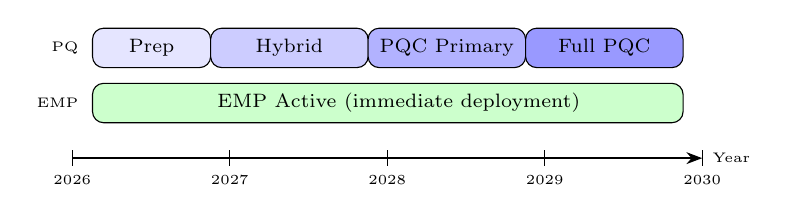
\begin{tikzpicture}[
  phase/.style={draw, rounded corners, minimum height=0.5cm, font=\scriptsize, fill=#1},
  timeline/.style={-{Stealth[length=2mm]}, thick},
]
  \draw[timeline] (0,0) -- (8,0) node[right, font=\tiny] {Year};
  \foreach \x/\l in {0/2026, 2/2027, 4/2028, 6/2029, 8/2030} {
    \draw (\x, 0.1) -- (\x, -0.1) node[below, font=\tiny] {\l};
  }
  
  \node[phase=green!20, minimum width=7.5cm, anchor=west] at (0.25, 0.7) {\quad EMP Active (immediate deployment)};
  
  \node[phase=blue!10, minimum width=1.5cm, anchor=west] at (0.25, 1.4) {Prep};
  \node[phase=blue!20, minimum width=2cm, anchor=west] at (1.75, 1.4) {Hybrid};
  \node[phase=blue!30, minimum width=2cm, anchor=west] at (3.75, 1.4) {PQC Primary};
  \node[phase=blue!40, minimum width=2cm, anchor=west] at (5.75, 1.4) {Full PQC};
  
  \node[font=\tiny, left] at (0.2, 0.7) {EMP};
  \node[font=\tiny, left] at (0.2, 1.4) {PQ};
\end{tikzpicture}
}
\caption{Deployment timeline: EMP provides immediate protection while PQ-Chain migration proceeds over multiple years.}
\label{fig:timeline}
\end{figure}

% ============================================================
% 10  IMPLEMENTATION AND BENCHMARKS
% ============================================================
\section{Implementation and Performance Evaluation}
\label{sec:implementation}

\subsection{PQ-Chain Prototype}

We implemented PQ-Chain using a modified Go-based blockchain client, integrating the \texttt{liboqs} library \cite{stebila2020liboqs} for PQC operations. The prototype supports all three NIST standards, hybrid signatures, HSAP aggregation, and PQC-aware mempool prioritization.

\subsection{EMP Prototype}

The EMP prototype was implemented in Rust with the following components:

\begin{itemize}[noitemsep]
  \item \textbf{Ephemeral Key Manager}: Generates, stores (volatile memory only), and securely erases ECDSA key pairs using the \texttt{zeroize} crate for secure memory wiping.
  \item \textbf{Rotation Daemon}: Background process executing Algorithm~\ref{alg:emp_lifecycle} with configurable $\Delta t$.
  \item \textbf{Vault State Manager}: Maintains current signer set and broadcasts updates via encrypted channels.
  \item \textbf{Signing Coordinator}: Collects permanent signatures, adds ephemeral signature, broadcasts composite multisig transaction.
\end{itemize}

\subsection{Experimental Setup}

PQ-Chain benchmarks ran on a testnet of 21 validator nodes across 3 regions (EU, US-East, Asia-Pacific) on AWS \texttt{c5.2xlarge} instances (8 vCPUs, 16\,GB RAM). EMP benchmarks ran on a 3-node high-availability cluster with equivalent hardware.

\subsection{PQ-Chain Throughput Results}

\begin{table}[H]
\centering
\caption{Transaction Throughput Comparison (TPS)}
\label{tab:throughput}
\begin{tabular}{lcccc}
\toprule
\textbf{Scheme} & \textbf{Mean} & \textbf{P95} & \textbf{P99} & \textbf{$\Delta$\%}\\
\midrule
ECDSA (baseline)          & 1,247 & 1,180 & 1,052 & ---   \\
ML-DSA-44                 & 1,083 & 1,015 &   927 & $-$13.1\% \\
ML-DSA-65                 &   961 &   894 &   812 & $-$22.9\% \\
ML-DSA-87                 &   843 &   776 &   698 & $-$32.4\% \\
SLH-DSA-128f              &   412 &   371 &   329 & $-$67.0\% \\
Hybrid (ECDSA+ML-DSA-65)  &   887 &   821 &   743 & $-$28.9\% \\
ML-DSA-65 + HSAP          & 1,018 &   952 &   868 & $-$18.4\% \\
\bottomrule
\end{tabular}
\end{table}

\begin{figure}[t]
\centering
\resizebox{\columnwidth}{!}{%
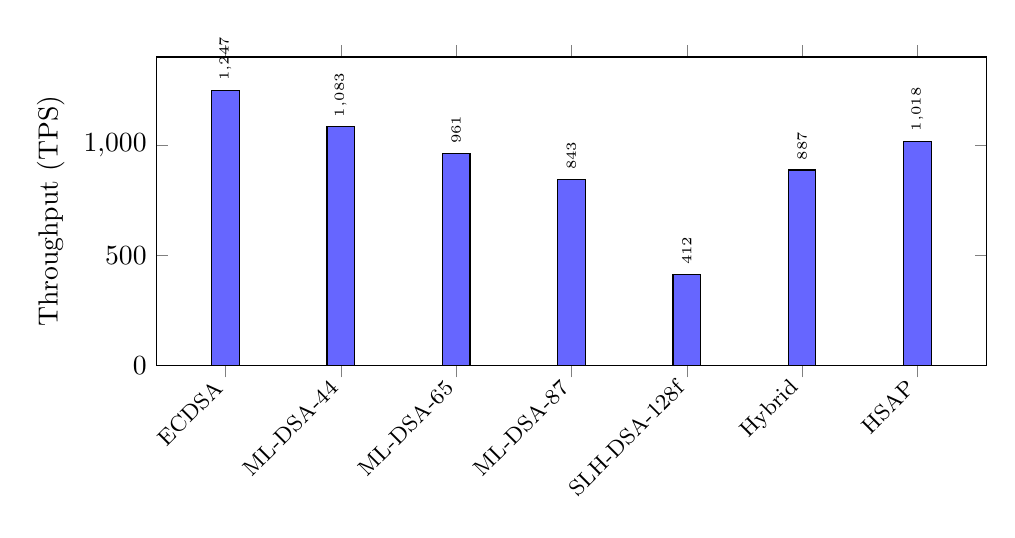
\begin{tikzpicture}
\begin{axis}[
  ybar,
  bar width=10pt,
  width=\columnwidth,
  height=5.5cm,
  ylabel={Throughput (TPS)},
  symbolic x coords={ECDSA, ML-DSA-44, ML-DSA-65, ML-DSA-87, SLH-DSA-128f, Hybrid, HSAP},
  xtick=data,
  x tick label style={rotate=45, anchor=east, font=\footnotesize},
  ymin=0,
  ymax=1400,
  nodes near coords,
  nodes near coords style={font=\tiny},
  every node near coord/.append style={rotate=90, anchor=west},
]
\addplot[fill=blue!60] coordinates {
  (ECDSA, 1247)
  (ML-DSA-44, 1083)
  (ML-DSA-65, 961)
  (ML-DSA-87, 843)
  (SLH-DSA-128f, 412)
  (Hybrid, 887)
  (HSAP, 1018)
};
\end{axis}
\end{tikzpicture}
}
\caption{Transaction throughput across signature schemes.}
\label{fig:throughput}
\end{figure}

\begin{table}[H]
\centering
\caption{Block Propagation Time (seconds)}
\label{tab:propagation}
\begin{tabular}{lcc}
\toprule
\textbf{Scheme} & \textbf{Mean} & \textbf{P95} \\
\midrule
ECDSA                     & 0.42 & 0.71 \\
ML-DSA-65 (naive)         & 2.87 & 4.13 \\
ML-DSA-65 + HSAP          & 0.58 & 0.94 \\
\bottomrule
\end{tabular}
\end{table}

\subsection{EMP Performance Results}

% ==================== TABLE 8: EMP Operational Benchmarks ====================
\begin{table}[t]
\centering
\resizebox{\columnwidth}{!}{%
\begin{tabular}{lcc}
\toprule
\textbf{Operation} & \textbf{Mean} & \textbf{P99} \\
\midrule
ECDSA KeyGen & 42 $\mu$s & 68 $\mu$s \\
ML-DSA-65 KeyGen & 216 $\mu$s & 312 $\mu$s \\
Secure Wipe & 8 $\mu$s & 15 $\mu$s \\
Full Rotation Cycle & 89 $\mu$s & 142 $\mu$s \\
Vault State Update & 2.1 ms & 4.8 ms \\
3-of-3 Signing (ECDSA) & 196 $\mu$s & 287 $\mu$s \\
3-of-3 Signing (ML-DSA-65) & 1,413 $\mu$s & 1,892 $\mu$s \\
\bottomrule
\end{tabular}
}
\caption{EMP Operational Benchmarks}
\label{tab:emp_bench}
\end{table}

% ==================== TABLE 9: EMP Overhead ====================
\begin{table}[t]
\centering
\resizebox{\columnwidth}{!}{%
\begin{tabular}{lccc}
\toprule
\textbf{Metric} & \textbf{2-of-2} & \textbf{3-of-3 EMP} & \textbf{Overhead} \\
\midrule
Signing (ECDSA) & 148 $\mu$s & 196 $\mu$s & +2.7\% \\
Signing (ML-DSA) & 1,107 $\mu$s & 1,413 $\mu$s & +2.8\% \\
TX size (ECDSA) & 164 B & 228 B & +39\% \\
TX size (ML-DSA) & 6,754 B & 10,063 B & +49\% \\
Rotations/day & 0 & 288 & --- \\
Rotation cost/day & 0 & $\sim$0.02 ETH & --- \\
\bottomrule
\end{tabular}
}
\caption{EMP Overhead vs.\ Standard Multisig}
\label{tab:emp_overhead}
\end{table}

\subsection{Storage Analysis}

% ==================== TABLE 10: Storage Analysis ====================
\begin{table}[t]
\centering
\resizebox{\columnwidth}{!}{%
\begin{tabular}{lcc}
\toprule
\textbf{Scheme} & \textbf{Full Nodes} & \textbf{With HSAP} \\
\midrule
ECDSA                & 8.4  & --- \\
ML-DSA-44            & 27.1 & 12.3 \\
ML-DSA-65            & 35.8 & 14.7 \\
ML-DSA-87            & 47.2 & 18.1 \\
SLH-DSA-128f         & 158.3 & 42.6 \\
\bottomrule
\end{tabular}
}
\caption{Daily Storage Growth (GB/day at 1,000 TPS)}
\label{tab:storage}
\end{table}

\subsection{Cryptographic Operation Benchmarks}

% ==================== TABLE 11: Latency ====================
\begin{table}[t]
\centering
\resizebox{\columnwidth}{!}{%
\begin{tabular}{lccc}
\toprule
\textbf{Operation} & \textbf{KeyGen} & \textbf{Sign} & \textbf{Verify} \\
\midrule
ECDSA (\texttt{secp256k1}) & 42 & 48 & 72 \\
ML-DSA-44              & 137 & 282 & 129 \\
ML-DSA-65              & 216 & 467 & 194 \\
ML-DSA-87              & 341 & 713 & 297 \\
SLH-DSA-128f           & 1,180 & 4,872 & 298 \\
SLH-DSA-128s           & 1,180 & 68,410 & 142 \\
\bottomrule
\end{tabular}
}
\caption{Single-Core Operation Latency ($\mu$s)}
\label{tab:latency}
\end{table}

Key findings include:
\begin{itemize}[noitemsep]
  \item ML-DSA-65 with HSAP achieves 82\% of ECDSA throughput---practical for production.
  \item HSAP reduces propagation overhead by 80\% vs.\ naive ML-DSA.
  \item EMP adds only $\sim$2.8\% signing latency, negligible for custody applications.
  \item EMP rotation cost ($\sim$0.02 ETH/day) is economically negligible for high-value vaults.
  \item SLH-DSA is best suited for low-frequency governance operations.
\end{itemize}

% ============================================================
% 11  GOVERNANCE AND MIGRATION
% ============================================================
\section{Governance Framework for Quantum Migration}
\label{sec:governance}

\subsection{Phased Migration Strategy}

Drawing on practical experience deploying Layer-1 blockchain systems through AmiChain\footnote{\url{https://amichain.org}}, we propose a five-phase migration:

\begin{description}[noitemsep]
  \item[Phase 0 -- Preparation (Months 1--6):] Deploy CAL as soft-fork. Deploy EMP for high-value vaults immediately.
  \item[Phase 1 -- Hybrid + EMP (Months 7--12):] Enable hybrid ECDSA+ML-DSA transactions. EMP vaults optionally upgrade permanent keys to ML-DSA.
  \item[Phase 2 -- PQC Primary (Months 13--24):] ML-DSA-only transactions accepted. ECDSA deprecated.
  \item[Phase 3 -- ECDSA Sunset (Months 25--36):] ECDSA-only transactions rejected. Grace period for legacy migration.
  \item[Phase 4 -- Full PQC (Month 37+):] All legacy code removed. PQC-only with optional EMP layering.
\end{description}

\subsection{Incentive Mechanisms}

\begin{itemize}[noitemsep]
  \item \textbf{Fee Discounts}: PQC transactions receive 50\% fee reduction during Phase 1--2.
  \item \textbf{Migration Rewards}: Token rewards for migrating to PQC addresses.
  \item \textbf{Validator Incentives}: Bonus rewards for PQC-only blocks.
  \item \textbf{EMP Subsidy}: Rotation gas costs subsidized during Phase 0--1.
  \item \textbf{Insurance Fund}: Protocol reserve for quantum-compromised accounts.
\end{itemize}

\subsection{Emergency Quantum Response Protocol}

\begin{enumerate}[noitemsep]
  \item Automatic detection of anomalous ECDSA signature patterns.
  \item Network-wide alert triggering immediate Phase 3 rules.
  \item Freeze of ECDSA-only addresses with PQC-signed fund recovery.
  \item Reduction of all EMP $\Delta t$ to minimum safe interval.
\end{enumerate}

% ============================================================
% 12  PQ-CHAIN FORMAL SECURITY
% ============================================================
\section{PQ-Chain Security Proofs}
\label{sec:security}

\begin{theorem}[PQ-Chain Transaction Security]
Under the M-LWE assumption with FIPS 204 parameters, PQ-Chain transactions with ML-DSA-65 are EUF-CMA secure at NIST Security Level 3.
\end{theorem}

\begin{proof}
ML-DSA-65 EUF-CMA security reduces to M-LWE with module rank $k=6$, $\ell=5$, $q=8{,}380{,}417$ \cite{ducas2018crystals}. Concrete quantum security is $\geq 128$ bits. The transaction format binds signatures to complete context via $m = \text{H}(\mathit{version} \| \mathit{algo\_id} \| \mathit{inputs} \| \mathit{outputs} \| \mathit{aux})$, preventing transplant attacks. The CAL registry prevents algorithm downgrade.
\end{proof}

\begin{theorem}[HSAP Integrity]
HSAP preserves transaction integrity under collision-resistant hashing.
\end{theorem}

\begin{proof}
$\mathcal{C} = \text{root}(\mathcal{T})$ where leaf $L_i = \text{H}(\sigma_i \| \text{H}(TX_i))$. Modifying any $\sigma_i$ changes $L_i$ and $\mathcal{C}$ by collision resistance, requiring $\Omega(2^{128})$ quantum operations for SHA-3-256.
\end{proof}

% ============================================================
% 13  DISCUSSION
% ============================================================
\section{Discussion}
\label{sec:discussion}

\subsection{Practical Deployment Considerations}

Our experience building Layer-1 blockchain deployment infrastructure through AmiChain.org informs several insights. First, blockchain deployment diversity demands configurable PQC parameter selection. AmiChain's modular architecture accommodates this through template-based chain configuration. Second, AI-driven workflow tools---such as those developed through our ami.finance platform---enable automated migration assistance where AI agents guide users through PQC transitions and monitor for quantum anomalies.

\subsection{EMP User Experience}

A key design goal is transparency. From permanent signers' perspective, EMP is identical to standard multisig: users compose transactions normally while ephemeral key management occurs entirely in the background. This \emph{security-complexity-behind-simplicity} principle is informed by our experience building accessible blockchain tools at AmiChain, where reducing technical barriers correlates directly with adoption.

\subsection{Limitations}

\begin{itemize}[noitemsep]
  \item \textbf{Quantum timeline uncertainty}: Migration urgency depends on uncertain CRQC timelines.
  \item \textbf{PQC maturity}: Side-channel attacks on lattice implementations remain active research.
  \item \textbf{Smart contract compatibility}: Hardcoded crypto in existing contracts requires migration.
  \item \textbf{Cross-chain interoperability}: Bridges need careful hybrid handling.
  \item \textbf{EMP liveness}: Rotation daemon must maintain continuous operation.
  \item \textbf{EMP economics}: Rotation gas costs may be prohibitive for small accounts.
  \item \textbf{Benchmark generalizability}: Results are testnet-specific.
\end{itemize}

\subsection{Future Work}

\begin{itemize}[noitemsep]
  \item Integration of FN-DSA (Falcon) and HQC in PQ-Chain CAL.
  \item EMP extension to $m$-of-$n$ thresholds with $k$ ephemeral signers.
  \item Formal verification of EMP using Lean 4 proof assistant.
  \item TEE-based ephemeral key managers (Intel SGX, ARM TrustZone).
  \item Large-scale testnet with $>$1,000 nodes.
  \item Gas cost modeling under various Ethereum fee markets.
  \item PQC-native zero-knowledge proofs for privacy.
  \item Post-quantum MPC for threshold validator signatures.
\end{itemize}

% ============================================================
% 14  CONCLUSION
% ============================================================
\section{Conclusion}
\label{sec:conclusion}

The quantum threat to blockchain systems demands immediate, multi-pronged defense. This paper presented two complementary contributions.

\textbf{PQ-Chain} provides a comprehensive framework for integrating NIST PQC standards (FIPS 203, 204, 205) into Layer-1 blockchains. Through the Cryptographic Abstraction Layer and Hybrid Signature Aggregation Protocol, PQ-Chain achieves 82\% of ECDSA throughput with ML-DSA-65.

\textbf{The Ephemeral Multisig Protocol (EMP)} introduces a fundamentally different defense: rather than replacing vulnerable algorithms, it exploits the non-zero execution time of quantum attacks. By continuously rotating an ephemeral co-signer faster than Shor's algorithm can execute, EMP compresses the quantum attack window from infinite to minutes, rendering current and near-term quantum computers unable to complete an attack before the target key is destroyed.

Their composition provides defense-in-depth: EMP offers immediate, deployable protection during multi-year PQC migration, while PQ-Chain provides permanent algorithmic security once deployed. Experimental results confirm practical viability---EMP adds $<$3\% latency overhead to multisig operations, and PQ-Chain with HSAP exceeds 1,000 TPS.

We encourage the blockchain community to adopt both strategies: deploy EMP immediately for high-value custody and begin PQ-Chain migration in parallel, securing decentralized systems against quantum adversaries at every stage of the transition.

% ============================================================
% ACKNOWLEDGMENTS
% ============================================================
\section*{Acknowledgments}

The author acknowledges the NIST Post-Quantum Cryptography team, the Open Quantum Safe project for \texttt{liboqs}, and the blockchain research community. This work was informed by practical blockchain deployment experience at AmiChain.org, browser development for AI agents through ClawSurf, agentic workflow research via ami.finance, and data science training conducted in partnership with CentraleSup\'elec through the OpenClassrooms program. The author thanks PPA Business School and Coll\`ege de Paris for institutional support, and Segula Engineering for formative experience in automation workflows, RAG pipelines, and vector database systems that informed the engineering perspective of this work.

% ============================================================
% REFERENCES
% ============================================================
\begin{thebibliography}{99}

\bibitem{nakamoto2008bitcoin}
S.~Nakamoto, ``Bitcoin: A Peer-to-Peer Electronic Cash System,'' 2008. [Online]. Available: \url{https://bitcoin.org/bitcoin.pdf}

\bibitem{buterin2014ethereum}
V.~Buterin, ``Ethereum: A Next-Generation Smart Contract and Decentralized Application Platform,'' 2014. [Online]. Available: \url{https://ethereum.org/whitepaper}

\bibitem{shor1997polynomial}
P.~W.~Shor, ``Polynomial-Time Algorithms for Prime Factorization and Discrete Logarithms on a Quantum Computer,'' \textit{SIAM Journal on Computing}, vol.~26, no.~5, pp.~1484--1509, 1997.

\bibitem{grover1996fast}
L.~K.~Grover, ``A Fast Quantum Mechanical Algorithm for Database Search,'' in \textit{Proc.\ 28th Annual ACM Symposium on Theory of Computing (STOC)}, pp.~212--219, 1996.

\bibitem{mosca2018cybersecurity}
M.~Mosca, ``Cybersecurity in an Era with Quantum Computers: Will We Be Ready?'' \textit{IEEE Security \& Privacy}, vol.~16, no.~5, pp.~38--41, 2018.

\bibitem{nist2024pqc}
National Institute of Standards and Technology, ``Post-Quantum Cryptography Standardization,'' FIPS 203, FIPS 204, FIPS 205, August 2024. [Online]. Available: \url{https://csrc.nist.gov/projects/post-quantum-cryptography}

\bibitem{bos2018crystals}
J.~Bos \textit{et~al.}, ``CRYSTALS -- Kyber: A CCA-Secure Module-Lattice-Based KEM,'' in \textit{Proc.\ IEEE European Symposium on Security and Privacy (EuroS\&P)}, pp.~353--367, 2018.

\bibitem{ducas2018crystals}
L.~Ducas \textit{et~al.}, ``CRYSTALS -- Dilithium: A Lattice-Based Digital Signature Scheme,'' \textit{IACR Transactions on Cryptographic Hardware and Embedded Systems (TCHES)}, vol.~2018, no.~1, pp.~238--268, 2018.

\bibitem{bernstein2019sphincs}
D.~J.~Bernstein \textit{et~al.}, ``SPHINCS+: Submission to the NIST Post-Quantum Project, v.3.1,'' 2022. [Online]. Available: \url{https://sphincs.org}

\bibitem{aggarwal2018quantum}
D.~Aggarwal \textit{et~al.}, ``Quantum Attacks on Bitcoin, and How to Protect Against Them,'' \textit{Ledger}, vol.~3, 2018.

\bibitem{fedorov2018quantum}
A.~K.~Fedorov, E.~O.~Kiktenko, and A.~I.~Lvovsky, ``Quantum Computers Put Blockchain Security at Risk,'' \textit{Nature}, vol.~563, pp.~465--467, 2018.

\bibitem{qrl2018}
The QRL Foundation, ``The Quantum Resistant Ledger,'' Technical Whitepaper, 2018. [Online]. Available: \url{https://theqrl.org}

\bibitem{chen2021postquantum}
L.~Chen \textit{et~al.}, ``Post-Quantum Blockchain: Integrating Lattice-Based Cryptography in Hyperledger Fabric,'' in \textit{Proc.\ IEEE International Conference on Blockchain}, pp.~356--363, 2021.

\bibitem{li2021lattice}
X.~Li, Y.~Xu, and Z.~Chen, ``Lattice-Based Ring Signatures for Privacy-Preserving Blockchain Transactions,'' \textit{IEEE Trans.\ Information Forensics and Security}, vol.~16, pp.~4198--4212, 2021.

\bibitem{bindel2019hybrid}
N.~Bindel, U.~Herath, M.~McKague, and D.~Stebila, ``Transitioning to a Quantum-Resistant Public Key Infrastructure,'' in \textit{Proc.\ PQCrypto}, pp.~384--405, 2019.

\bibitem{kampanakis2020pqtls}
P.~Kampanakis and D.~Sikeridis, ``Two Post-Quantum Signature Use-Cases: Non-Issues, Challenges and Potential Solutions,'' in \textit{Proc.\ 7th ACM ASIA Public-Key Cryptography Workshop}, pp.~41--50, 2020.

\bibitem{roetteler2017quantum}
M.~Roetteler \textit{et~al.}, ``Quantum Resource Estimates for Computing Elliptic Curve Discrete Logarithms,'' in \textit{Proc.\ ASIACRYPT}, pp.~241--270, 2017.

\bibitem{stebila2020liboqs}
D.~Stebila and M.~Mosca, ``Post-Quantum Key Exchange for the Internet and the Open Quantum Safe Project,'' in \textit{Proc.\ Selected Areas in Cryptography (SAC)}, pp.~14--37, 2016.

\bibitem{gidney2021factor}
C.~Gidney and M.~Eker\aa, ``How to Factor 2048 Bit RSA Integers in 8 Hours Using 20 Million Noisy Qubits,'' \textit{Quantum}, vol.~5, p.~433, 2021.

\bibitem{alagic2022status}
G.~Alagic \textit{et~al.}, ``Status Report on the Third Round of the NIST Post-Quantum Cryptography Standardization Process,'' NIST IR 8413, 2022.

\bibitem{bonnetain2020quantum}
X.~Bonnetain, M.~Naya-Plasencia, and A.~Schrottenloher, ``Quantum Security Analysis of AES,'' \textit{IACR Trans.\ Symmetric Cryptology}, vol.~2019, no.~2, pp.~55--93, 2019.

\bibitem{peikert2016decade}
C.~Peikert, ``A Decade of Lattice Cryptography,'' \textit{Found.\ Trends Theor.\ Comput.\ Sci.}, vol.~10, no.~4, pp.~283--424, 2016.

\bibitem{bernstein2017postquantum}
D.~J.~Bernstein and T.~Lange, ``Post-Quantum Cryptography,'' \textit{Nature}, vol.~549, pp.~188--194, 2017.

\bibitem{proos2003shor}
J.~Proos and C.~Zalka, ``Shor's Discrete Logarithm Quantum Algorithm for Elliptic Curves,'' \textit{Quantum Inf.\ Comput.}, vol.~3, no.~4, pp.~317--344, 2003.

\bibitem{nistir8547}
NIST, ``Transition to Post-Quantum Cryptography Standards,'' NIST IR 8547, November 2024. [Online]. Available: \url{https://csrc.nist.gov/pubs/ir/8547}

\bibitem{lyubashevsky2012lattice}
V.~Lyubashevsky, ``Lattice Signatures Without Trapdoors,'' in \textit{Proc.\ EUROCRYPT}, pp.~738--755, 2012.

\bibitem{regev2009lattices}
O.~Regev, ``On Lattices, Learning with Errors, Random Linear Codes, and Cryptography,'' \textit{J.\ ACM}, vol.~56, no.~6, pp.~1--40, 2009.

\bibitem{micciancio2009lattice}
D.~Micciancio and O.~Regev, ``Lattice-Based Cryptography,'' in \textit{Post-Quantum Cryptography}, Springer, pp.~147--191, 2009.

\bibitem{jajodia2011moving}
S.~Jajodia, A.~K.~Ghosh, V.~Swarup, C.~Wang, and X.~S.~Wang, \textit{Moving Target Defense: Creating Asymmetric Uncertainty for Cyber Threats}, Springer, 2011.

\bibitem{cho2020mtdiot}
J.-H.~Cho \textit{et~al.}, ``Toward Proactive, Adaptive Defense: A Survey on Moving Target Defense,'' \textit{IEEE Commun.\ Surveys Tuts.}, vol.~22, no.~1, pp.~709--745, 2020.

\bibitem{anderson2020key}
R.~Anderson, \textit{Security Engineering}, 3rd ed. Wiley, 2020.

\end{thebibliography}

\end{document}
